\section{Methodology}
\subsection{Methodology}
\begin{frame}{Methodology}
  \small
  \setbeamertemplate{enumerate item}{\Roman{enumi}}
  \begin{block}{Steps}
    \begin{enumerate}%[label=\bfseries Step \Roman*]
      %\renewcommand{\labelenumii}{Task \arabic{enumii}:}
      \item \textbf{Research on the characteristics of data delivered by sensors, in this case the GPS receiver.}

        % It can bring theoretical fundaments to improve the representation of data, for example achieving data compression.
        Identify special characteristics of GPS data that may trigger the study of techniques like outliers elimination, noise reduction, filtering, windowing, and framing to launch pre-processing of data delivered by sensors.

        % \begin{enumerate}
        %   \item Research on characteristics of data delivered by GPS receiver.
        % \end{enumerate}

      \item \label{itm:def-sel-mob-pttrns} \textbf{Definition and selection of mobility patterns to be identified.}

        This step is needed to identify the target mobility patterns that will be employed later in the pattern identifier element.

        % Examples of these mobility patterns are static, walking, running, vehicle at high speed, etc.

        The set of target mobility patterns defined here will be part of the input for the pattern identifier element.

        % \begin{enumerate}
        %   \setcounter{enumii}{1}
        %   \item Coding a sample app to gather GPS data from the smartphone.
        %   This app will access GPS receiver in a continuous and permanent way.
        %   \item Analysis of data delivered by the mobile app.
        %   \item Selection of the mobility patterns that will be recognized by the platform.
        %   \item Creation of the formal definition of mobility pattern.
        % \end{enumerate}
    \end{enumerate}
  \end{block}
\end{frame}

\begin{frame}{Methodology}
  \small
  \setbeamertemplate{enumerate item}{\Roman{enumi}}
  \begin{block}{Steps}
    \begin{enumerate}
      \setcounter{enumi}{2}
      \item \label{itm:research-alg-pttrn-rec} \textbf{Research and adaptation of algorithms to detect mobility patterns of user based on data delivered by GPS.}

        % Once the characteristics of data collected by sensors have been studied and the patterns to be identified have been defined, it is needed to detect a mobility pattern from these data.
        
        The pattern is helpful to get information about user's context and therefore in the generation of policies.
        
        The selected algorithms should consider the constraints present in mobile devices.

        % \begin{enumerate}
        %   \setcounter{enumii}{5}
        %   \item Research on algorithms for pattern recognition from GPS data.
        %   \item Definition of metrics for evaluating algorithms.
        %   \item Evaluation of algorithms.
        %   \item Selection of proper algorithm(s), discussing the best conditions for its (their) usage.
        % \end{enumerate}

      \item \textbf{Creation of the pattern identifier element (PIE).}

        This element must identify the pattern from data collected by sensors by employing the algorithm(s) selected in the Step \ref{itm:research-alg-pttrn-rec}.
        
        The pattern identified must be included in the set of mobility patterns defined in the Step \ref{itm:def-sel-mob-pttrns}.

        % \begin{enumerate}
        %   \setcounter{enumii}{9}
        %   \item Definition of parameters accepted by the PIE and their formal representation.
        %   \item Elaboration of the PIE.
        %   % \item Fine tunning of the PIE towards its usage in a constrained device (the smartphone)
        % \end{enumerate}

    \end{enumerate}
  \end{block}
\end{frame}

\begin{frame}{Methodology}
  \small
  \setbeamertemplate{enumerate item}{\Roman{enumi}}
  \begin{block}{Steps}
    \begin{enumerate}
      \setcounter{enumi}{4}

      \item \textbf{Creation of the policy generator element (PGE).}

        It includes the definition of a formal representation of policies.
        
        This policy generator element will obtain the duty cycle that the GPS receiver must implement to perform the next GPS reading.

        % \begin{enumerate}
        %   \setcounter{enumii}{11}
        %   \item Definition of parameters accepted by the PGE and their representation.
        %   \item Creation of the formal definition of \emph{policy}.
        %   \item Elaboration of the PGE.
        %   % \item Fine tunning of the PGE towards its usage in a constrained device (the smartphone)
        % \end{enumerate}

      \item \textbf{Development of a software element (SE) that integrates both PIE and PGE.}

        This software element will be implemented in the Android platform.
        
        % The Android platform is selected in this research because of its popularity, well documented SDK, and because its availability in the research center.

        % \begin{enumerate}
        %   \setcounter{enumii}{14}
        %   % \item Analysis and definition of logical elements involved in software abstractions.
        %   \item Definition of SE architecture.
        %   \item Research on Android API for specialized components related to sensor access and task-process management.
        %   \item Coding of the SE.
        % \end{enumerate}

      \item \textbf{Experimentation.}

        Key aspects are precision and energy saving.
        
        % Precision refers to the fidelity that data collected by employing policies maintain in relation to actual ground truth data.
        % This can be measured by executing data analysis processes over data collected by sensors through policies versus data collected without employing policies.
        
        % Energy saving refers to the reduction in the energy consumption that is obtained when applying policies versus the inter-built facilities of mobile operating systems.
        
        This step involves the definition of experiments and the development of mobile applications that employs the constructed software element.

        % \begin{enumerate}
        %   \setcounter{enumii}{17}
        %   \item Definition of experiments targeting energy saving and user tracking precision metrics.
        %   \item Development of mobile apps employing the SE for running the experimentation.
        %   \item Execution of the experimentation.
        %   \item Results analysis.
        % \end{enumerate}

    \end{enumerate}
  \end{block}
\end{frame}


\begin{frame}{Methodology}
  \begin{block}{Basic idea of proposed method}
    \begin{figure}
      \centering
      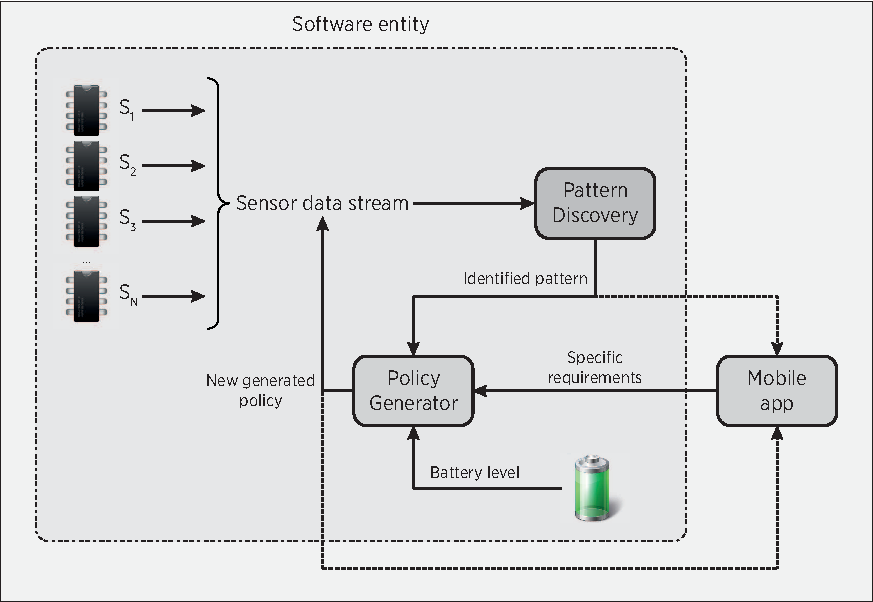
\includegraphics[scale=0.45]{methodology-stages}
      \caption[Methodology workflow]{Workflow described by the proposed methodology}
      \label{fig-methodology-workflow}
    \end{figure}
  \end{block}
\end{frame}